\begin{onehalfspace}

\chapter{Gliederung und Zeitplan}

\begin{figure}[H]
	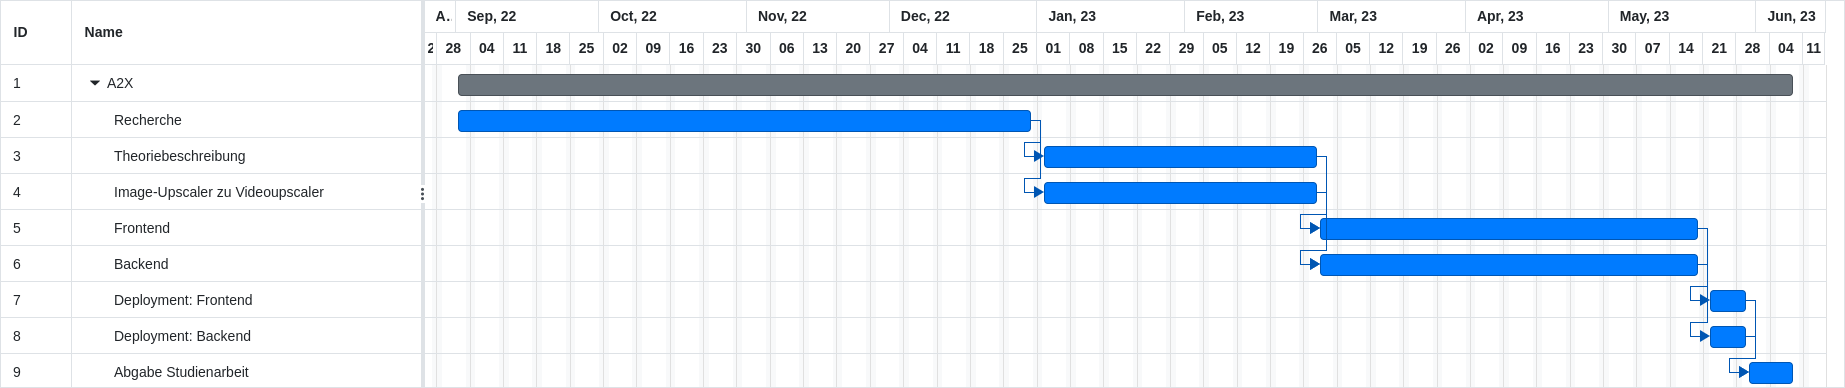
\includegraphics[width=\textwidth]{Bilder/Gantt}
\end{figure}

\begin{center}
	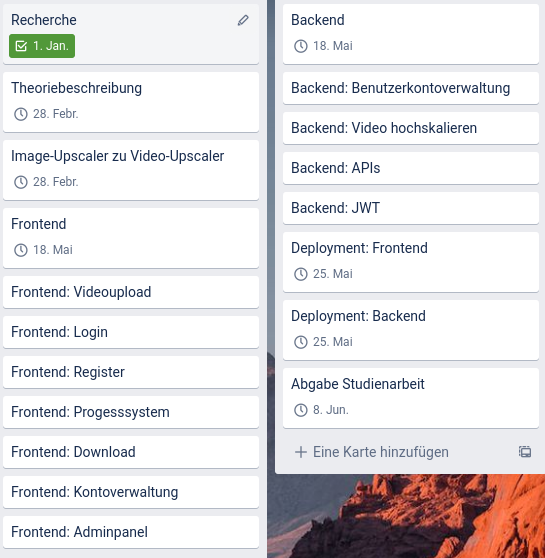
\includegraphics[height=10cm]{Bilder/Trello}
\end{center}

Eine grobe Gliederung lässt sich daraus herausarbeiten:

\begin{itemize}
	\item Abstract
	\item Einleitung
	Aktuelle Situation
	Problemstellung
	
	\item Theoretischer Hintergrund
	\begin{itemize}
		\item Upscaler
		\item Website
		\begin{itemize}
			\item Backend
			\item Frontend
		\end{itemize}
	\end{itemize}
	
	\item Umsetzung
	\begin{itemize}
		\item Upscaler
		\item Website
		\begin{itemize}
			\item Backend
			\item Frontend
		\end{itemize}
	\end{itemize}
	
	\item Fazit
	\item Ausblick
	
\end{itemize}


\end{onehalfspace}
